\documentclass[10pt]{article}
\usepackage{amsmath}
\usepackage{setspace}
\usepackage{hyperref}
\usepackage[pdftex]{graphicx}

\setlength{\textheight}{9in} \setlength{\topmargin}{-.5in}
\setlength{\textwidth}{6.5in} \setlength{\oddsidemargin}{0in}
\setlength{\evensidemargin}{0in}

\title{COMP220 - Code::Blocks Project Setup}
\author{ }
\date{Fall 2015}

\begin{document}
\maketitle

Previously we used a suite of mostly GNU tools to develop build our programs.  Now we're using the Integrated Development Environment (IDE) \textit{Code::Blocks} to manage the development of our code. Like all IDEs, Code::Blocks (C::B) provides an all-in-one solution that includes a text editor, integration with compilers, integration with debuggers, and build management. There are several basic things we need to be able to do.  You may recall them from working with \textit{make} in Comp161.
\begin{itemize}
\item Link external libraries with our code
\item Compile the gTest executable for our unit tests
\item Compile a debugging version of our program that works with the integrated debugger. 
\item Compile a release (ready for users) version of our program. 
\end{itemize}
The last two items on this list will happen by default when we create new projects in Code::Blocks. The first two require our intervention. This document walks you through the basic setup for projects in the course. 

\section{Where are your documents?}

In C::B you organize programs into projects. Projects are grouped by workspaces. You can have only one workspace open and active at once. You can have multiple projects/programs open but only one can be active. It's name will be in bold text. Workspaces correspond to folders on your hard dive and projects correspond to sub-folders of the workspace folder. When you add source documents to your project, then they can be found within the project folder. The exact location off the folder is specified when you create the project and the workspace folder is specified when you first start up C::B. You'll be submitting source code only for this course, so it's important that you know where these things are located. Pay attention as you set things up.

\section{Global Settings and C++11}

Before you start creating projects and source documents, it's useful to know where your global compiler settings are and how to change them. These settings let you set some gcc compiler options that will be applied to every single build of every single project unless you say otherwise. In our case there is only one option we want to be applied globally and that's to compile with respect to the C++11 standard. 


Go to the \textit{Settings} drop-down menu and select \textit{Compiler...} and you should now see this window modulo some selections:

\vspace{.1in}
\begin{center}
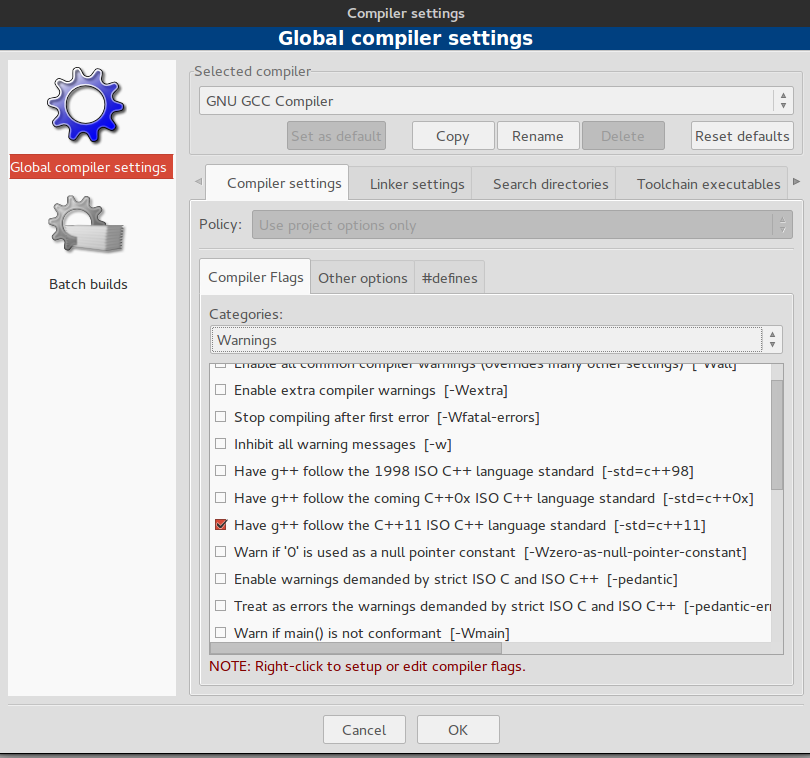
\includegraphics[scale=.5]{CB_GlobalCompiler.png}
\end{center}
\vspace{.1in}

Take a moment to browse some of the options. 	All we're concerned with is setting the C++11 compiler, which has been done in the above image. You can more easily browse flags by selecting a filter category in the \textit{Categories} drop-down. As you can see above, the \textit{Warnings} category has been selected. In here we find the different C++ standards along with the familiar warnings flags like \textit{-Wall}.  We'll reserve \textit{-Wall} for our debugging builds rather than apply it to all the builds. When you're ready, check the box for C++11 and press OK to close the window.

\section{Basic Project}

Now we're going to setup a basic project for a dead simple hello world program. 

\subsection{Create a new Empty Project}

First we make a new project by either going to \textit{File $>$ New $>$ Project...} or by using the \textit{New File} button under the drop down menu.  In either case, we're greeted with the following:

\vspace{.1in}
\begin{center}
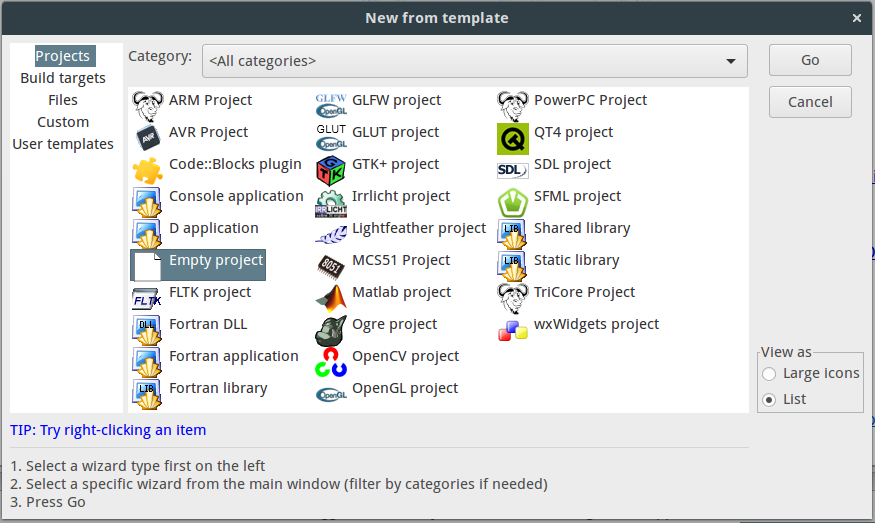
\includegraphics[scale=.5]{CB_NewProject.png}
\end{center}
\vspace{.1in}

As is done in the picture, select the \textit{Empty Project} option and then press the \textit{Go} button. Now you'll see the Empty Project window where you pick the project name and location. Go ahead and fill this out, paying attention to the locations, and press \textit{Next}. The next screen lets you set the compiler and choose some default builds. We want all the default options, as shown below.


\vspace{.1in}
\begin{center}
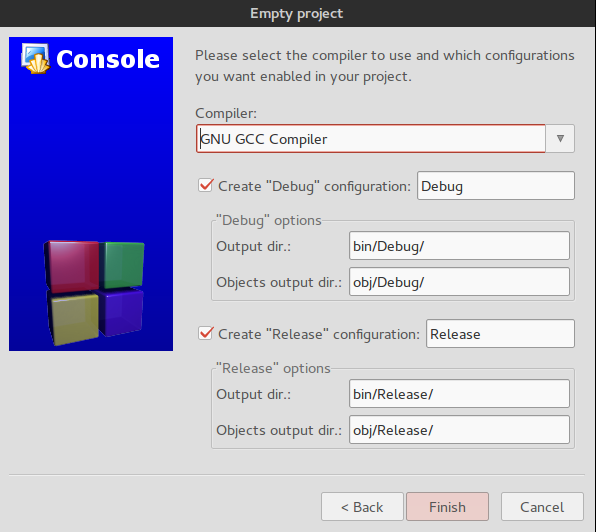
\includegraphics[scale=.5]{CB_EmptyProjectBuilds.png}
\end{center}
\vspace{.1in}

So, if your window looks like the one above, press enter. 

\subsection{Set Some Build Specific Compiler Options}

Before we move on, we're going to make sure our Debug and Release builds have the options enabled that we want. To change build options you can right click on the project name in the workspace explorer and select \textit{Build Options...}. You should make sure to select the options shown in the following two images. Be sure to notice which build is selected and the category filters.

\vspace{.1in}
\begin{center}
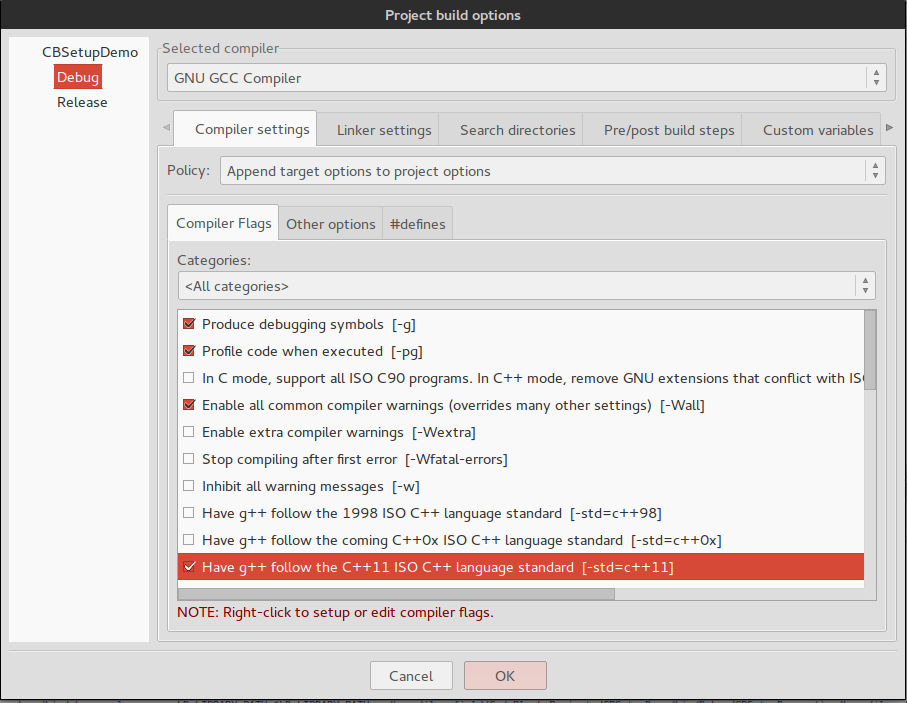
\includegraphics[scale=.5]{CB_BasicDebugOpts.png}
\end{center}
\vspace{.1in}

\vspace{.1in}
\begin{center}
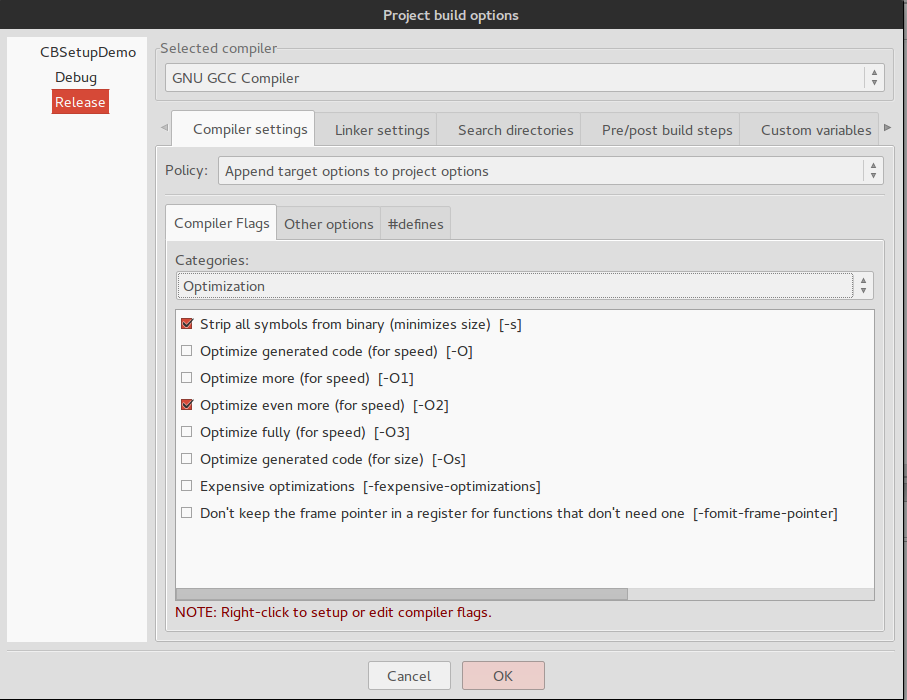
\includegraphics[scale=.5]{CB_BasicReleaseOpts.png}
\end{center}
\vspace{.1in}

\subsection{Adding a Source Document}

Now we want to create a file called \textit{HelloWorld.cpp} in a folder named \textit{src} within our project folder. By keeping our source documents organized into \textit{src} we make it easier manage code submission later. You can either go ahead and create the \textit{src} folder using the GUI or CLI or you'll have the change to do it when you create your first project file.

First go back to the \textit{New} options either from the File menu or the New File button and select the new file option. You want to select the empty file option as shown below.

\vspace{.1in}
\begin{center}
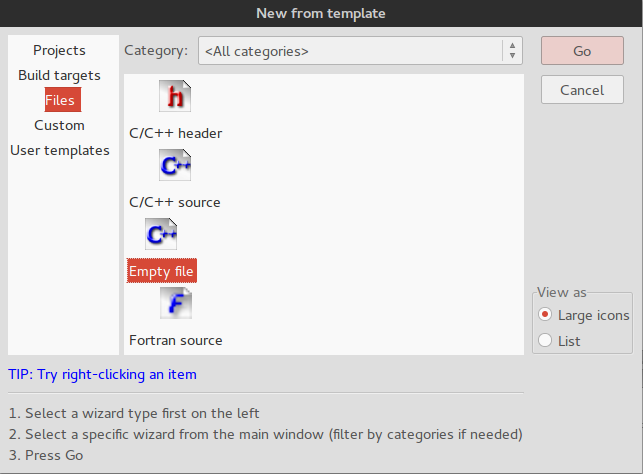
\includegraphics[scale=.5]{CB_NewFileEmptyCPP.png}
\end{center}
\vspace{.1in}

Once you select the file type, Empty in this case, you'll be able to choose the name and location as well as which builds should include the file. You are required to enter the full path to the file. This can be a bit of pain to type out but if you select the \textit{...} button next to the text field you should start the file browser in your project directory. You can then browse to the directory of your choosing and enter your desired file name. This is the time where you can create a \textit{src}folder if you have not done so already. If this document is a library document or contains your main procedure, then it's probably included in all the builds, like we see here. 

\vspace{.1in}
\begin{center}
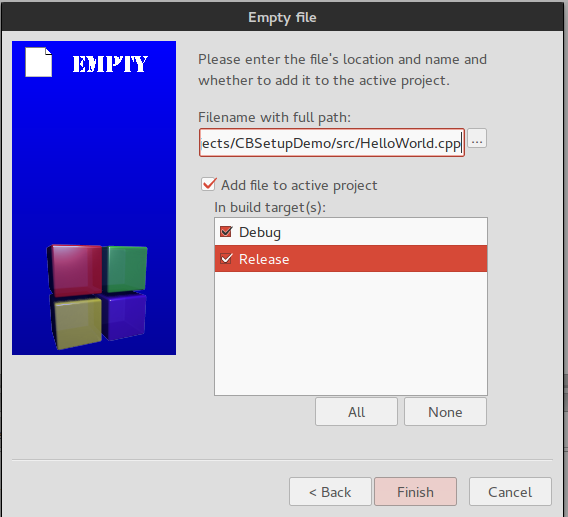
\includegraphics[scale=.5]{CB_NewFileEmptyName.png}
\end{center}
\vspace{.1in}

Once your file has been created it should pop up in the text editor. If not, you can select it from the project explorer. Go ahead and write up some kind of dead simple program, like this hello world you see here. 

\vspace{.1in}
\begin{center}
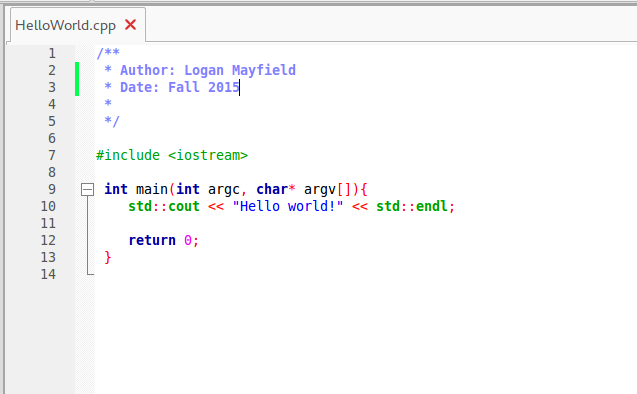
\includegraphics[scale=.5]{CB_HelloWorld.png}
\end{center}
\vspace{.1in}

\subsection{Building and Running}

You should notice a few things: C::B will highlight things it things are syntax errors and attempt to auto-complete code for you. This can save a tone of time and we'll keep an eye out for these kind of features as we work more with C::B. What we need to know now is:
\begin{itemize}
\item How to select a build type
\item How to compile
\item How to run the compiled program
\end{itemize}

You should see the follow items on the bar above the editor.
\vspace{.1in}
\begin{center}

\includegraphics[scale=.5]{CB_BuildBar.png}
\end{center}
\vspace{.1in}

The drop-down on the right lets you select the build, we'll work mostly in Debug as its setup for more, better warnings and debugging/profiling. The gear button will compile the code. The green play button runs the code. If no compiled version of the build exists, then hitting run prompts you to build or not. Finally the gear/play combo will build and then run. The blue arrows in a circle will force the rebuilding of all files in the project. Each of these buttons has a corresponding menu option in the \textit{Build} drop down. There's also a \textit{Clean} option in that menu that will clear out temp files just like we did with our makefiles.

Compiler and errors and warnings will appear down below the text editor. The compiled program itself will be in the project folders corresponding to the build type. Your encouraged to introduce some errors to your hello world program, play around a bit and just explore C::B a bit before moving on to the more involved stuff to come.   

\newpage
\section{Adding a Testing Build for gTests}

We develop code with Google's gTest unit test library. Tests are written in a file separate from the library they're testing and, when compiled, are linked to a pre-written main procedure provided by Google. To enact this in C::B we need to create a whole new Build type that includes the test code and links to the necessary libraries. 

First, let's add the Build to the project. Get to project \textit{Properties} either through the Project drop down or by right clicking the project name. Once there, select the \textit{Build Targets} tab and press the \textit{Add} button. I named my build \textit{gTests} but you can name in just \textit{Tests} or something similar if you wish.  What we're going to do is basic set the Build up like Debug and Release by filling in the options as follows:

\vspace{.1in}
\begin{center}
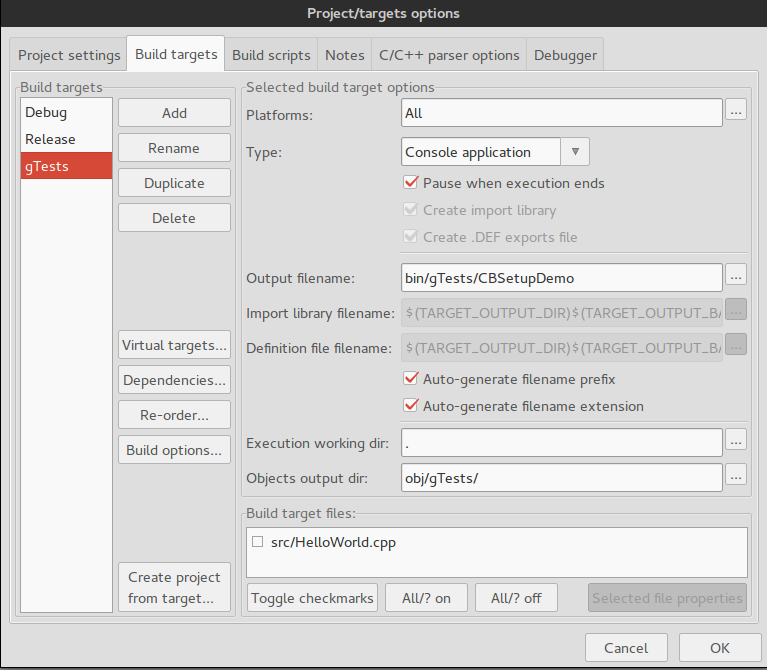
\includegraphics[scale=.5]{CB_TestBuildSetup.png}
\end{center}
\vspace{.1in}

Once you've got your basic build setup, we need to add the link options for the Google libraries. You can get to the build options from the previous window by selecting the \textit{Build Options} button.  Once there, select your new testing build and select the \textit{Linker Settings} tab.  Then add the three link flags like you see here:

\vspace{.1in}
\begin{center}
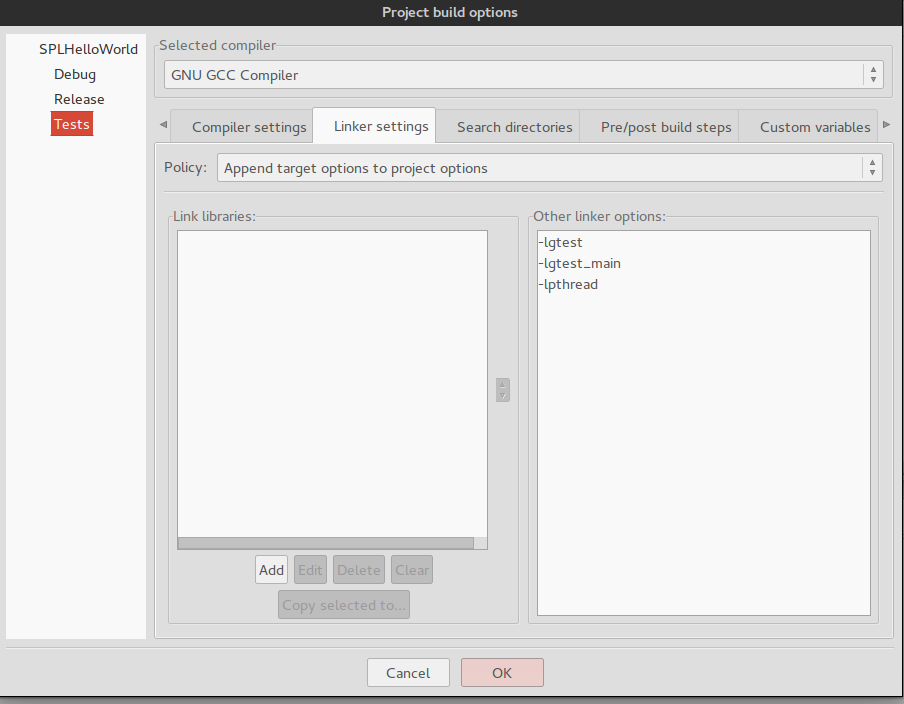
\includegraphics[scale=.5]{CB_TestLinkOpts.png}
\end{center}
\vspace{.1in}

Our test build is setup. Now we need tests!

\subsection{ Adding Tests Files }

Let's just say I have the file \textit{HelloTests.cpp} already in my project \textit{src} folder and I want it to be compiled with my testing build. Then we can simply return to the Build Targets tab in our Project's Properties window and check the box for the test file like you see here.

\vspace{.1in}
\begin{center}
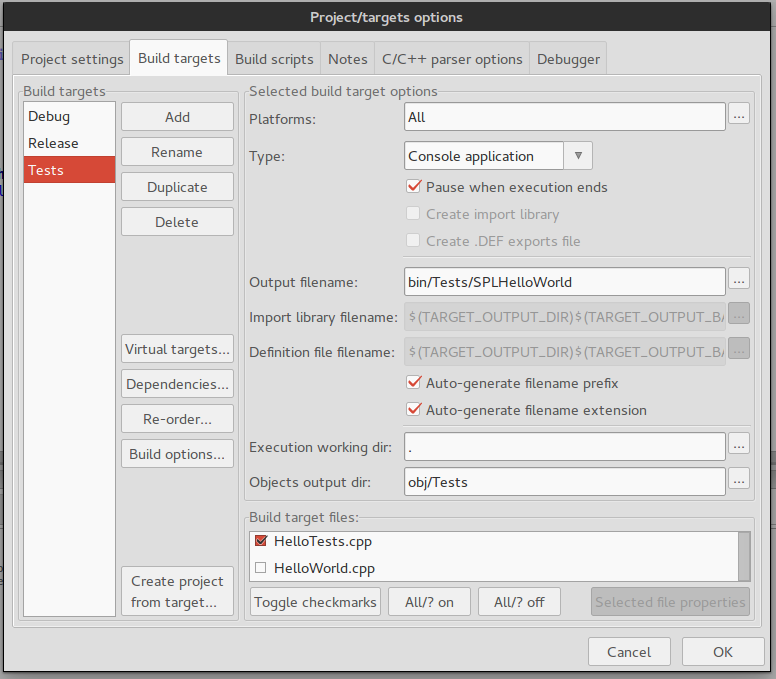
\includegraphics[scale=.5]{CB_TestFileSelect.png}
\end{center}
\vspace{.1in}

Alternatively, when we create new files, we got to choose to which builds they're added. So, if you're starting from a fresh, empty file for your tests and your test build is already setup, then you can choose to add them to the test build when you create the file. Just remember that tests builds generally include your tests and the libraries your testing but not any files containing another main. On the other hand, your Debug and Release builds should not build tests and should definitely build some main other than the Google testing main. 


\section{Conclusion}

You now know how to setup a basic C++ project in C::B and can configure a testing build to work with the Google gTest unit testing framework. You'll find the file \textit{comp220-cbsetupdemo.zip} in the course home directory (/home/comp220/fa15).  It contains a simple hello world program and a simple gTest test set. Feel free to use it to practice setting up a project before you get to your first assignments. Either way, try to walk through these steps at least once before you start your first lab assignment.



\end{document}